\documentclass[fleqn,10pt]{olplainarticle}
% Use option lineno for line numbers 

\title{COMSM0104: Web Technologies 2019\\Final Assignment Report}
\author[1]{Tao Xu}
\author[2]{Yinan Yang}
\affil[1]{si19010@bristol.ac.uk}
\affil[2]{ff19085@bristol.ac.uk}

\keywords{Vue, SQLite}

\begin{abstract}
	Our two-person team consists of Tao Xu (si19010) and Yinan Yang (ff19085). Due to environmental influences, we used a remote collaboration model via GitHub to co-develop this project.
	
 We have created a website that generates resumes. Our website is based on Vue's front-end technical architecture, taking advantage of Vue's MVVM, the Model-View- ViewModel, we have done it to componentize the front-end development.
\end{abstract}

\begin{document}
	
	\flushbottom
	\maketitle
	\thispagestyle{empty}
	
	\section*{Introduction}
	
We have created a website that generates resumes called Simple Resume Maker. The website provides basic user registration and login functionality. Once logged in, the user can edit the resume template provided on the website on the web page and download a .pdf version of the resume.
	
	\section*{Self-Evaluation}
	
	Guidelines can be included for standard research article sections, such as this one.
	
	\subsection*{HTML}
	\subsection*{CSS}
	\subsection*{JS}
	\subsection*{PNG}
	\subsection*{SVG}
	\subsection*{Server}
	\subsection*{Database}
	\subsection*{Dynamic pages}

	
	\section*{CSS}
	\label{sec:examples}
	
	Use section and subsection commands to organize your document. \LaTeX{} handles all the formatting and numbering automatically. Use ref and label commands for cross-references.
	
	\subsection*{JS}
	
	Use the table and tabular commands for basic tables --- see Table~\ref{tab:widgets}, for example. You can upload a figure (JPEG, PNG or PDF) using the project menu. To include it in your document, use the includegraphics command as in the code for Figure~\ref{fig:view} below.
	
	\begin{figure}[ht]
		\centering
		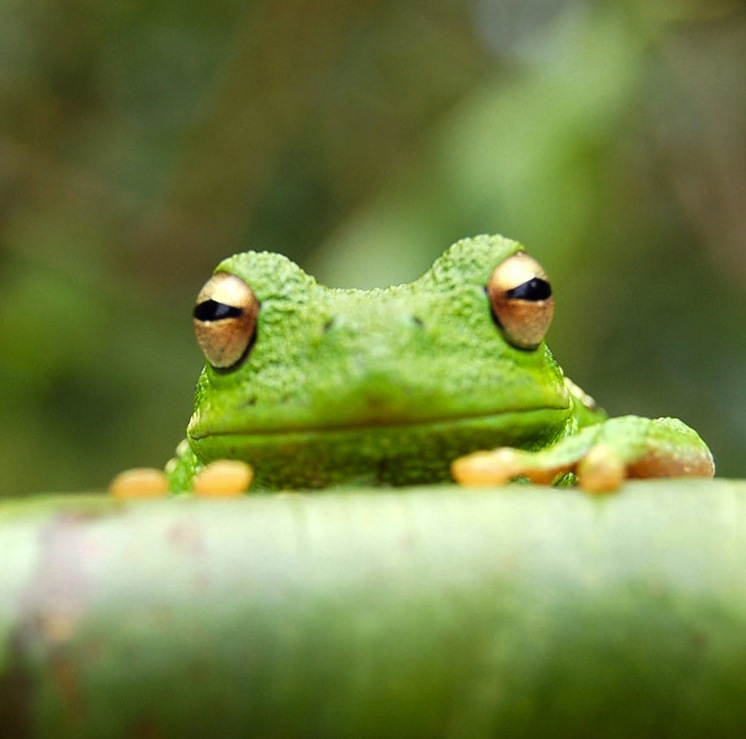
\includegraphics[width=0.7\linewidth]{frog}
		\caption{An example image of a frog.}
		\label{fig:view}
	\end{figure}
	
	\begin{table}[ht]
		\centering
		\begin{tabular}{l|r}
			Item & Quantity \\\hline
			Candles & 4 \\
			Fork handles & ?  
		\end{tabular}
		\caption{\label{tab:widgets}An example table.}
	\end{table}
	
	\subsection*{Citations}
	
	LaTeX formats citations and references automatically using the bibliography records in your .bib file, which you can edit via the project menu. Use the cite command for an inline citation, like \cite{lees2010theoretical}, and the citep command for a citation in parentheses \citep{lees2010theoretical}.
	
	\subsection*{Mathematics}
	
	\LaTeX{} is great at typesetting mathematics. Let $X_1, X_2, \ldots, X_n$ be a sequence of independent and identically distributed random variables with $\text{E}[X_i] = \mu$ and $\text{Var}[X_i] = \sigma^2 < \infty$, and let
	$$S_n = \frac{X_1 + X_2 + \cdots + X_n}{n}
	= \frac{1}{n}\sum_{i}^{n} X_i$$
	denote their mean. Then as $n$ approaches infinity, the random variables $\sqrt{n}(S_n - \mu)$ converge in distribution to a normal $\mathcal{N}(0, \sigma^2)$.
	
	\subsection*{Lists}
	
	You can make lists with automatic numbering \dots
	
	\begin{enumerate}[noitemsep] 
		\item Like this,
		\item and like this.
	\end{enumerate}
	\dots or bullet points \dots
	\begin{itemize}[noitemsep] 
		\item Like this,
		\item and like this.
	\end{itemize}
	\dots or with words and descriptions \dots
	\begin{description}
		\item[Word] Definition
		\item[Concept] Explanation
		\item[Idea] Text
	\end{description}
	
	\section*{Acknowledgments}
	
	Additional information can be given in the template, such as to not include funder information in the acknowledgments section.
	
	\bibliography{sample}
	
\end{document}